\section{Evaluation}
\label{sec:eval}

In this section, our benchmark is the CNN/Daily
Mail DMQA dataset~\cite{HermannKGEKSB15,NallapatiZSGX16,SeeLM17}
\footnote{https://cs.nyu.edu/˜kcho/DMQA/},
consisting of pairs of a single source document and a multi-sentence summary.
The dataset includes 286,817 training pairs,
13,368 validation pairs and 11,487 test pairs.
%\tabref{table:cnn} shows an example pair from training data.
We follow the same pre-processing step used by \citet{SeeLM17},
and fill in the blanks with answer named entities.
We show an example of such pairs in \tabref{tab:gold_a}.

We compare our length constrained summarization model with
the basic CNN seq2seq model and the state-of-the-art
length controllable summarization model \cite{abs-1711-05217}
\footnote{All datasets, source code and generated summaries
can be downloaded from \url{http://202.120.38.146/sumlen}.}. 
Following Fan et al.,
we distribute the dataset into a set of disjoint buckets that
correspond to summaries of different lengths. Each 
bucket contains roughly equal number of documents.  
The distribution is shown in \figref{fig:buckets}.

\begin{figure}[th!]
\centering
\scalebox{1.0}{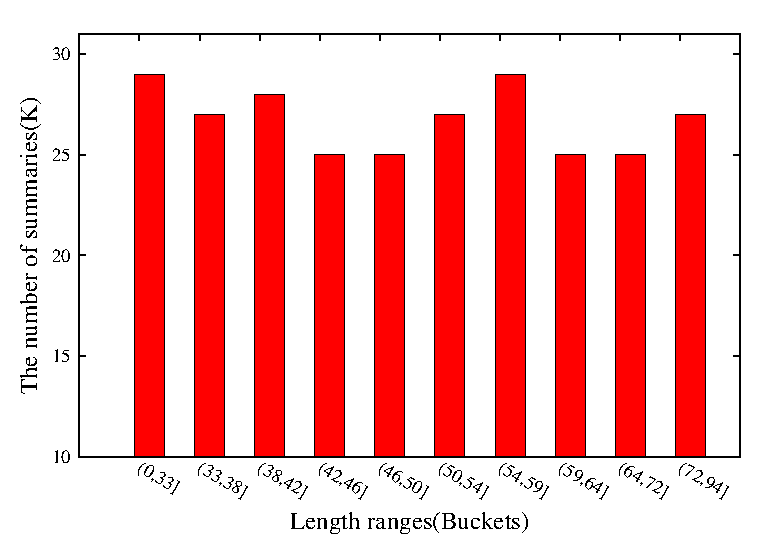
\includegraphics[width=1.0\columnwidth]{data_LRC.eps}}
\caption{The buckets distribution of the dataset} \label{fig:buckets}
\end{figure}

All competing methods
have three flavors: {\em free}, {\em truncated} and {\em exact}.
In the free version(Free), given the desired length $N$,
each method generates summaries naturally until
an EOS is generated. 
%And we limit the length of generated 
%summaries to 100.\footnote{The maximum length of summaries in CNN/DailyMail dataset is 94.}
%This version usually generates
%more complete and fluent summaries.
In the truncated version(Trunc), each method artificially
inserts an EOS if EOS has not been generated in the first $N$ tokens.
In the exact version(Exact), each method
generates $N$ non-EOS tokens by assigning a score
of -$\infty$ to the EOS and inserts an EOS after the $N$-th token.
%\KZ{How do u make sure that no EOS is generated in the first N tokens
%for all three methods?}
The purpose of Free version is to evaluate the method's ability to
generate summaries with desired length; the purpose of the other
two versions is to enable fair comparison of the summaries in terms of
their content given that the summaries are of equal length. 
%Whereas the performance of Trunc and Exact version shows the effectiveness 
%of a method to generate readable summaries with the length constraint.


%We include similarity as a metric to evaluate the
%ability of semantic generation of the output.

%ROUGE scores tend to favor longer summaries.
%Therefore, we compute ROUGE scores
%on both the naturally produced summary (without truncation)
%and the summary after truncating
%to the desired length or the max length of a length range.


\subsection{Experimental Setup}
In the following experiments, 
all the competing models have 8 convolutional layers in
both encoder and decoder parts with kernel width as 3.
For each convolutional layer, 
we set the hidden vector size as 512 and the embedding size as 256.
To alleviate the overfitting problem,
we add the dropout ($p=0.2$) layer for 
all convolutional layers and fully connected layers.

%Following Gehring et al. 
%\shortcite{gehring2017convs2s,abs-1711-05217},
To optimize the proposed model,
we use Nesterov's
accelerated gradient method \cite{SutskeverMDH13} with gradient clipping 0.1 \cite{PascanuMB13}, momentum 0.99,
and learning rate 0.2.
We terminate the training process when the learning rate drops below $10e$-$5$.
We set beam size as 5 for the beam search algorithm in the testing step.
%For testing, we use beam search algorithm with the beam size 5.
%
%For length control model without penalty, we distribute the training set into a set of buckets which denote different length range. Each buchets does not overlap with other buckets and contains roughly an equal number of documents. For
%
Next, we introduce the evaluation metrics in the following experiments:
\begin{enumerate}
\item \textit{ROUGE} scores (F1 score) of the produced
summaries, including ROUGE-1(R-1), ROUGE-2(R-2) and
ROUGE-L(R-L)~\cite{rouge-a-package-for-automatic-evaluation-of-summaries}.
ROUGE-2 is the most popular metric for summarization.

\item \textit{Variance}(Var) of the summary lengths against
the desired length $len$:
%The variance is computed as following:
\begin{equation}
var = 0.001 * \frac{1}{n}\sum_{i=0}^{n} |l_i - len|^2, 
\end{equation}
where $n$ is the number of pairs in the dataset, and $l_i$ is the length of
the generated summary $i$. 
We introduce the variance to evaluate the
ability of exact control of the output length.

\item \textit{Similarity}(Sim) between generated summaries
and their corresponding reference summaries:
\begin{equation}
sim = \frac{1}{n}\sum_{i=0}^{n} \frac{y_{i}\cdot y'_{i}}{||y_{i}|| ||y'_{i}||}
\end{equation}
where $n$ is the number of pairs. 
%\KZ{
$y_i$ is
the vector representation of the reference summary $i$ and $y'_{i}$ is 
vector of the corresponding generated summary $i$.
%We compute $y_i$ and $y'_i$ by the 
Both $y_i$ and $y'_i$ are the sum of
GloVe~\footnote{https://nlp.stanford.edu/projects/glove/.} word vectors of
the words in these summaries. 
%Is it really averaging?} 
% More specifically, the similarity is computed as following:
%For length range $(l, r]$, we define the length error of the $i$-th pair as follows:
%\begin{equation}
%e_i = max\{0, max\{(r-x_i), (x_i-l)\}-R\},
%\end{equation}
%where $R$ is the range length (i.e. $r-l$) and $x_i$ denotes the actual length of
%the generated summary.
%We include the similarity metric because, when the desired length is very different
%from the gold length, the ROUGE scores may not reflect the true quality of the
%generated summaries. \KZ{We compute the similarity by ...}
\end{enumerate}

We introduce the similarity metric here to complement the ROUGE scores
because \citet{Yao} showed that the standard ROUGE scores cannot capture semantic similarity
beyond n-grams. Given the same source document, abstractive summarization may
create summaries that don't share many words but mean the same.
%This causes the generated summary not to match the target 
%summary word by word. Therefore, we introduce the similarity metric which reflects 
%the semantic information of the generated summary. 
To show the effectiveness of this Sim metric, we design a dataset
from the summarization tasks of TAC 2010$\sim$2011\footnote{https://tac.nist.gov/}.
The TAC dataset consists of 90 topics in total, each with 2 
subset. Each subset has 4 reference summaries 
by different humans. We assume reference summaries about the same topic to be
semantically similar to each other, while summaries across topics are unrelated.
Thus we created 2,160 pairs of similar summaries as postive data and 2,160 pairs of
unrelated summaries as negative data.
We then compute the Pearson correlation between the ROUGE score and the
ground truth as well as between Sim and the ground truth and show
the results in \tabref{table:pearson}. Sim metric certainly resembles semantic
similarity better than ROUGE by this experiment.
%There are 46 topics in TAC 2010 and 44 topics in TAC 2011. 
%Each topic has 4 reference summaries.
%We design a new dataset consisting of summary pairs from above summaries.
%We set that the semantic score of summaries from same topic and different 
%topics is 1 and 0. Each summary respectively has 3 corresponding summaries in 
%same topic and different topics. So we can get a (0,1) distribution
%of semantic score for TAC 2010$\sim$2011 as ground tuth. Then we compute the
%ROUGE score and similarity score based on these
%summary pairs. Compared with ground truth, we get Pearson correlation coefficient of ROUGE and
%similarity metric. As shown in \tabref{table:pearson}, similarity metric gets closer to the ground truth.
%
\begin{table}[th]
	\small
	\centering
	\caption{Pearson correlation with the true semantic relatedness}
	\label{table:pearson}
	\begin{tabular}{lcccc}
		\hline
		& TAC 2010 & TAC 2011  \cr
		\hline
		R-2 & 0.6107 & 0.6034  \cr
		Sim & \bf 0.6653& \bf 0.7165  \cr
		\hline
	\end{tabular}
\end{table}

In this paper, we don't use manual evaluation as the major
metric. The reason is that \citet{rouge-a-package-for-automatic-evaluation-of-summaries}
showed that the manual evaluation is unstable and the inter-human agreement is 
low due to the variety in abstractive summaries. The ROUGE scores and 
Similarity scores can respectively measure the syntactic similarity 
and semantic similarity. They are complementary to each other
and give better quantitative assessment of the summarization quality. 

\subsection{Experiment 1: Gold Summary Lengths}
\label{sec:exp1}

%In this part, we design different experiments to compare our models with basic model (CNN) and state of art model\citep{abs-1711-05217}.

In the first experiment, for each test document-summary pair, we set the desired length as the length of the gold summary
and ask the competing methods to generate a summary
with the desired length. As shown 
in \tabref{table:gold}, the proposed model (LC)
%consistently 
outperforms the other models on all of the evaluation metrics.
The ROUGE score shows the accuracy of these models.
Lower variance reflects better length control of the model.
Higher similarity reflects better quality of generated summaries from the semantic 
point of view.
%Furthermore, our models can generate better summaries which have the setting length.

\begin{table}[ht]
	\small
	\centering
	\caption{Desired Length: Gold Summary Lengths}
	\label{table:gold}
	%\begin{tabular}{lcccccccc}
	\begin{tabular}{p{0.3em}p{0.3em}p{1.8em}<{\centering}p{1.8em}<{\centering}p{1.8em}<{\centering}p{2.2em}<{\centering}p{2.2em}<{\centering}}%{|p{7cm}|rl|}}
		\hline
		\multicolumn{2}{c}{}                                                     & R-1 & R-2 & R-L & Var & Sim \\ \hline
		\multicolumn{1}{l|}{\multirow{3}{*}{Free}} &
		\multicolumn{1}{l|}{CNN} & 34.49 & 14.38 & 25.78 & 0.3465 & 0.9220 \\ \cline{2-7}
		\multicolumn{1}{c|}{}                        & \multicolumn{1}{l|}{Fan} & 34.53 & 14.40 & 25.78 & 0.3446 & 0.9216 \\ \cline{2-7}
		\multicolumn{1}{c|}{}                        & \multicolumn{1}{l|}{LC} & \bf 35.45 & \bf 14.50 & \bf 26.02 & \bf 0.0005 & \bf 0.9272\\ \cline{2-7}
        \hline
		\multicolumn{1}{l|}{\multirow{3}{*}{Trunc}} &
		\multicolumn{1}{l|}{CNN} & 34.76 & \bf 14.53 & 26.00 & 0.3045 & 0.9201 \\ \cline{2-7}
		\multicolumn{1}{c|}{}                        & \multicolumn{1}{l|}{Fan} & 34.74 & 14.52 & 25.97 & 0.3031 & 0.9197 \\ \cline{2-7}
		\multicolumn{1}{c|}{}                        & \multicolumn{1}{l|}{LC} & \bf 35.44 & 14.48 & \bf 26.02 & \bf 0.0002 & \bf 0.9268\\ \cline{2-7}
        \hline
		\multicolumn{1}{l|}{\multirow{3}{*}{Exact}} &
		\multicolumn{1}{l|}{CNN} & 35.39 & 14.43  & \bf 26.07 & 0.0 & 0.9249 \\ \cline{2-7}
		\multicolumn{1}{c|}{}                        & \multicolumn{1}{l|}{Fan} & 35.37 & 14.42 & 26.03 & 0.0 & 0.9246 \\ \cline{2-7}
		\multicolumn{1}{c|}{}                        & \multicolumn{1}{l|}{LC} & \bf 35.44 & \bf 14.50 & 26.02 & 0.0 & \bf 0.9268 \\ \cline{2-7}
		\hline
	\end{tabular}
\end{table}

The LC model achieves the highest ROUGE and similarity scores
as well as the lowest variance
in both Free and Exact version,
which shows the effectiveness of LC for generating 
high quality summaries under length constraint. 
In the Trunc version, the LC model outperforms the other 
comparable models on all evaluation metrics
except for the ROUGE score.
%In the Free version and Exact version, the ROUGE score and similarity score of LC model is the highest,
%and the variance of LC model is lowest. It means that we can control generated summary length best
%without lossing sematic information. 
%In the Trunc vesion, LC model is still the best on variance evaluation and 
%similarity evalution except the ROUGE score. 
%Comparing ROUGE scores of each model on different versions, we can
%find that our score is stable. It means that LC model can generate summaries in desired length without using any
%auxiliary method of controlling length. 
Note that, the ROUGE scores of LC model are
very stable, indicating its effective length control.
As for the other two models, 
they have better ROUGE score on Trunc version. 
However, as the example shown in 
\tabref{table:gold_example}\footnote{The entities in different color 
indicate two important roles in the text. The words in bold type mean correct 
content.}, higher ROUGE scores do not necessarily mean 
high quality abstractive summaries. 
%However, as the Pearson correlation coefficient shown in 
%\tabref{table:pearson} and the example shown in 
%\tabref{table:gold_example}\footnote{The entities 
%in different color indicate two important roles in the text. 
%The words in bold type mean correct content.},
%we argue that the similarity score is more reasonable 
%to measure the quality of generated summary 
%for the abstractive summarization on the
%sematic level. 

\begin{table*}[th!]
\begin{center}
\caption{Example summaries generated in Experiment 1.}
\label{table:gold_example}
\small
\subtable[Source document and reference summary (36 tokens)]{
        \label{tab:gold_a}
        \begin{tabular}{lclc}%{|p{7cm}|rl|}
        \hline \bf Source document \\
        \hline the last time \color{green}{frank jordan} \color{black}{spoke with his son,} \color{red} {louis jordan} 
		       \color{black}{was fishing on \textbf{a sailboat a few miles off the south}}\\
			   \textbf{carolina coast}. the next time ... more than two months had passed and the younger jordan was on a contrainer\\
			   ship 200 miles from north carolina, just \textbf{rescued from his disabled boat} .
			   ``\textbf{i thought i lost you},''the relieved\\ 
			   father said. louis jordan, 37, took his sailboat out 
			   in \textbf{late january} and \textbf{hadn't been heard from in 66 days} ... the\\
			   \color{red}{younger jordan} \color{black}{said
			   \textbf{he took his sailboat out to the gulf stream to find some better fishing} ... the boat capsized} \\
			   two more times before he was \textbf{rescued}, according to jordan.\\
		\hline \bf Reference summary \\
        \hline \color{red}{louis jordan} \color{black}{says his sailboat capsized three times . 
		       he \textbf{survived} by collecting  rainwater and eating raw fish .}\\
			   \color{green}{frank jordan} \color{black}{told cnn \textbf{his son} is n't an experienced sailor but has a strong will .}\\
		\hline
        \end{tabular}
        }
\qquad
\subtable[Free summary(29 tokens), Trunc summary(29 tokens) and Exact summary of CNN]{
        \label{tab:gold_b}
        %\begin{tabular}{lcccccccc}
	    \begin{tabular}{p{1.5em}<{\centering}p{1.5em}<{\centering}p{26.5em}|p{1.4em}<{\centering}p{1.4em}<{\centering}p{1.4em}<{\centering}p{1.5em}<{\centering}p{2.0em}<{\centering}p{2.0em}<{\centering}}%{|p{7cm}|rl|}
      	\hline
		\multicolumn{2}{c}{}& Summary & R & P & F & Var & Sim  \\ \hline
		\multicolumn{1}{c|}{\multirow{4}{*}{CNN}} &
		\multicolumn{1}{c|}{Free} & \tabincell{l}{\color{green}{frank jordan} 
		                                           \color{black}{\textbf{took his sailboat out to the gulf stream to find some}} \\ 
												   \textbf{better fishing} , jordan says . `` it took so long , '' jordan says . \\
												   } 
		& 6.06 & 9.09 & 7.27 & 0.049 & 0.9217 \\ \cline{2-8}
		\multicolumn{1}{c|}{}                        & 
		\multicolumn{1}{c|}{Trunc} & \tabincell{l}{\color{green}{frank jordan} 
		                                           \color{black}{\textbf{took his sailboat out to the gulf stream to find some}} \\ 
												   \textbf{better fishing} , jordan says . `` it took so long , '' jordan says . \\
												   } 
		& 6.06 & \bf 9.09 & 7.27 & 0.049 & 0.9217 \\ \cline{2-8}
		\multicolumn{1}{c|}{}                        & 
		\multicolumn{1}{c|}{Exact} & \tabincell{l}{\color{green}{frank jordan} 
		                                           \color{black}{\textbf{took his sailboat out to the gulf stream to find some}}\\
		                                           \textbf{better fishing} , jordan says . jordan says he took his sailboat out \\
												   to the gulf stream to find some better fishing .\\
													} 
		& 6.06 & \bf 6.25 & 6.15 & - & 0.9254 \\ \cline{2-8}
        \hline
        \end{tabular}
        }
\qquad
\subtable[Free summary(50 tokens), Trunc summary(36 tokens) and Exact summary of Fan]{
        \label{tab:gold_c}
        %\begin{tabular}{lccccccc}
	    \begin{tabular}{p{1.5em}<{\centering}p{1.5em}<{\centering}p{26.5em}|p{1.4em}<{\centering}p{1.4em}<{\centering}p{1.4em}<{\centering}p{1.5em}<{\centering}p{2.0em}<{\centering}p{2.0em}<{\centering}}%{|p{7cm}|rl|}
      	\hline
		\multicolumn{2}{c}{}& Summary & R & P & F & Var & Sim  \\ \hline
		\multicolumn{1}{c|}{\multirow{4}{*}{Fan}} &
		\multicolumn{1}{c|}{Free} & \tabincell{l}{\color{green}{frank jordan}
		                                          \color{black}{\textbf{took his sailboat out to the gulf stream to find some}} \\
		                                           \textbf{better fishing .} jordan says he took his sailboat out to the gulf \\
												   stream to find some better fishing . jordan says he took his sailboat \\
												   out to the gulf stream to find some better fishing .\\
		                                          }  
		& 6.06 & \bf 4.35 & 5.06 & 0.196 & 0.9215 \\ \cline{2-8}
		\multicolumn{1}{c|}{} & 
		\multicolumn{1}{c|}{Trunc} & \tabincell{l}{\color{green}{frank jordan}
		                                           \color{black}{took his sailboat out to the gulf stream to find some} \\
		                                           better fishing . \textbf{his son} , \color{red}{louis jordan}
												   \color{black}{\textbf{took his sailboat out to the}}\\
												   \textbf{gulf stream to find some better fishing .}\\
		                                           } 
		& 12.12 & \bf 12.90 & 12.50 & 0.0 & 0.9194\\ \cline{2-8}
		\multicolumn{1}{c|}{} & 
		\multicolumn{1}{c|}{Exact} & \tabincell{l}{\color{green}{frank jordan}
		                                           \color{black}{took his sailboat out to the gulf stream to find some} \\
		                                           better fishing . \textbf{his son} , \color{red}{louis jordan} 
												   \color{black}{\textbf{took his sailboat out to the }}\\
												   gulf stream to find some \textbf{better fishing .}\\
		                                           } 
		& 12.12 & 12.90 & 12.50 & - & 0.9194\\ \cline{2-8}
        \hline
        \end{tabular}
        }
\qquad
\subtable[Free summary(36 tokens), Trunc summary(36 tokens) and Exact summary of LC(ours)]{
        \label{tab:gold_d}
        %\begin{tabular}{lccccccc}
	    \begin{tabular}{p{1.5em}<{\centering}p{1.5em}<{\centering}p{26.5em}|p{1.4em}<{\centering}p{1.4em}<{\centering}p{1.4em}<{\centering}p{1.5em}<{\centering}p{2.0em}<{\centering}p{2.0em}<{\centering}}%{|p{7cm}|rl|}
      	\hline
		\multicolumn{2}{c}{} & Summary & R & P & F & Var & Sim  \\ \hline
		\multicolumn{1}{c|}{\multirow{4}{*}{LC}} &
		\multicolumn{1}{c|}{Free} &  \tabincell{l}{\color{red}{louis jordan} 
		                                            \color{black}{was on \textbf{a sailboat a few miles off the}}
		                                            \textbf{south carolina }\\
													\textbf{coast} . he \textbf{had n't been heard from in 66 days} 
													when he was \\
													\textbf{rescued} . he was \textbf{rescued from his boat} .\\
		                                           }
		& 6.06 & 6.06 & 6.06 & 0.0 & \bf 0.9293 \\ \cline{2-8}
		\multicolumn{1}{c|}{}                        & 
		\multicolumn{1}{c|}{Trunc} &  \tabincell{l}{\color{red}{louis jordan} 
		                                            \color{black}{was on \textbf{a sailboat a few miles off the}}
		                                            \textbf{south carolina }\\
													\textbf{coast} . he \textbf{had n't been heard from in 66 days} 
													when he was \\
													\textbf{rescued} . he was \textbf{rescued from his boat} .\\
		                                           }
		& 6.06 & 6.06 & 6.06 & 0.0 & \bf 0.9293 \\ \cline{2-8}
		\multicolumn{1}{c|}{}                        & 
		\multicolumn{1}{c|}{Exact} &  \tabincell{l}{\color{red}{louis jordan} 
		                                            \color{black}{was on \textbf{a sailboat a few miles off the}}
		                                            \textbf{south carolina}\\
													\textbf{coast} . he \textbf{had n't been heard from in 66 days} 
													when he was \\
													\textbf{rescued} . he was \textbf{rescued from his boat} .\\
		                                           }
		& 6.06 & 6.06 & 6.06 & - & \bf 0.9293 \\ \cline{2-8}
        \hline
        \end{tabular}
        }
\end{center}
\end{table*}
The ROUGE score consists of Recall(R), Precision(P) and F1-measure(F). 
The summary tends to achieve a better ROUGE score 
when the length of generated summary is slightly shorter than 
the desired length.
%, since the tokens generated in the first are usually more preciser.
%However, such ROUGE score can not 
%reflect the semantic information of the summary.
%although it has the problem of the lack of 
%the semantic information.
In \tabref{tab:gold_b}, 
the CNN model has the same R score 
as LC model and a higher P score than LC model because of its slightly
shorter length.  
We can see that the CNN model achieve a higher F score even its generated summary is not good. 
Moreover, for the basic model,
the generated summary always repeats the sentences
when the length of generated summary is longer than the desired length.
In \tabref{tab:gold_c}, 
the P score of its Trunc version would be improved
by a large margin.
%As shown in \tabref{tab:gold_c}, its P score grows up by a large margin from Free version to Trunc version. 
Thus, the ROUGE score for the Trunc version biases toward
the models with weak length control.
%So the Trunc version is advantageous to the model which can 
%not control the summary length well.
The generated summaries of the LC model in \tabref{tab:gold_d}, 
which capture the semantic of the reference summary and 
satisfy the constraint length very well,
are better than the other two models even with a slightly lower ROUGE score.
%contains the most information of source documents and satisfies the gold length.
%We can see that the generated summary of LC model is
%better than other two but our ROUGE score is slightly lower. 
The topic of this example is that Louis Jordan, who is the son of Frank Jordan, 
got lost during sailing and was finally rescued from his boat. 
Our model generates the summary with correct
information, but other two models get the Louis Jordan and Frank Jordan mixed up.
This is correctly measured by the similarity scores. 
%Similarity score is more reasonable to measure the quality of generated summary.


\subsection{Experiment 2: Arbitrary Lengths}

In the second experiment, we ask the methods to generate
summaries with arbitrary lengths. 
We report the results of all three methods with five arbitrary lengths: 10, 30, 50, 70 and 90.
%We test the models on several arbitrary desired lengths:
%10, 30, 50, 70 and 90.
%have different border in the same distance. And (0,10],(0,20] and (0,30] have different distance of range.
%Our length range control methods can handle point lengths by setting
%both the min and max value of the input range to be the desired length.
We show the performance of each model with different
length constraints in \tabref{table:arbi}, \tabref{table:arbiSim}, \figref{fig:Sim} and \figref{fig:var}.
The basic CNN model has the same ROUGE scores in the Free version since it cannot control the length of generated 
summaries on its own.
%, we the summaries it produces are automatically truncated at the max of the desired
%length
%length range or the desired length.
For \citet{abs-1711-05217}, the desired length is mapped to
the model's predefined fixed length range(s) that {\em contains}
the desired length before it produces its summaries. For example,
the desired length $10$ is mapped to the first bucket $(0, 33]$.
%The ROUGE scores of Fan model in Free 10 and Free 30 are the same.

\begin{table*}[th]
	\centering
	\small
	\caption{Desired Length: 10, 30, 50, 70, 90}
	\label{table:arbi}
    \subtable[\textbf{Free} version]{
	    \begin{tabular}{p{1.8em}<{\centering}p{1.8em}<{\centering}p{1.8em}<{\centering}p{1.8em}<{\centering}p{1.8em}<{\centering}p{1.8em}<{\centering}p{1.8em}<{\centering}p{1.8em}<{\centering}p{1.8em}<{\centering}p{1.8em}<{\centering}p{1.8em}<{\centering}p{1.8em}<{\centering}p{1.8em}<{\centering}p{1.8em}<{\centering}p{1.8em}<{\centering}p{1.8em}<{\centering}}%{|p{7cm}|rl|}
		\hline
		\multirow{2}{*}{Free}&
		\multicolumn{3}{c}{10}&\multicolumn{3}{c}{30}&\multicolumn{3}{c}{50}&\multicolumn{3}{c}{70}&\multicolumn{3}{c}{90}\cr
		\cmidrule(lr){2-4} \cmidrule(lr){5-7} \cmidrule(lr){8-10} \cmidrule(lr){11-13} \cmidrule(lr){14-16}
		& CNN & Fan & LC & CNN & Fan & LC & CNN & Fan & LC & CNN & Fan & LC & CNN & Fan & LC \cr
		\hline
		R-1 & \bf34.49 & 34.28 & 19.03 & \bf34.49 & 34.28 & 32.26 & 34.49 & 34.60 & \bf34.71 & 34.49 & \bf34.65 & 33.83 & \bf34.49 & 30.56 & 32.17 \cr
		R-2 & \bf14.38 & 14.18 & 8.45  & \bf14.38 & 14.18 & 13.60 & 14.38 & \bf14.41 & 14.24 & 14.38 & \bf14.50 & 13.67 & \bf14.38 & 12.20 & 13.00 \cr
		R-L & \bf25.78 & 25.60 & 16.47 & \bf25.78 & 25.60 & 24.64 & 25.78 & \bf25.79 & 25.62 & 25.78 & \bf25.82 & 24.67 & \bf25.78 & 22.08 & 23.28 \cr
		\hline
        \end{tabular}
        }
     \subtable[\textbf{Trunc} version]{
	    \begin{tabular}{p{1.8em}<{\centering}p{1.8em}<{\centering}p{1.8em}<{\centering}p{1.8em}<{\centering}p{1.8em}<{\centering}p{1.8em}<{\centering}p{1.8em}<{\centering}p{1.8em}<{\centering}p{1.8em}<{\centering}p{1.8em}<{\centering}p{1.8em}<{\centering}p{1.8em}<{\centering}p{1.8em}<{\centering}p{1.8em}<{\centering}p{1.8em}<{\centering}p{1.8em}<{\centering}}%{|p{7cm}|rl|}
		\hline
		\multirow{2}{*}{Trunc}&
		\multicolumn{3}{c}{10}&\multicolumn{3}{c}{30}&\multicolumn{3}{c}{50}&\multicolumn{3}{c}{70}&\multicolumn{3}{c}{90}\cr
		\cmidrule(lr){2-4} \cmidrule(lr){5-7} \cmidrule(lr){8-10} \cmidrule(lr){11-13} \cmidrule(lr){14-16}
		& CNN & Fan & LC & CNN & Fan & LC & CNN & Fan & LC & CNN & Fan & LC & CNN & Fan & LC \cr
		\hline
		R-1 & \bf20.14 & 20.12 & 18.77 & 32.96 & \bf32.99 & 32.25 & 35.14 & 35.07 & \bf35.60 & 34.49 & \bf34.67 & 33.83 & 31.27 & \bf34.70 & 32.16 \cr
		R-2 & \bf9.27 & 9.22 & 8.31 & \bf14.06 & 14.04 & 13.60 & \bf14.46 & 14.40 & 14.30 & 14.38 & \bf14.50 & 13.67 & 12.40 & \bf14.55 & 13.00 \cr 
		R-L & \bf17.35 & 17.34 & 16.28 & \bf25.11 & 25.06 & 24.62 & \bf26.09 & 26.05 & 25.90 & 25.78 & \bf25.82 & 24.67 & 22.69 & \bf25.86 & 23.29 \cr
		\hline
        \end{tabular}
        }
     \subtable[\textbf{Exact} version]{
	    \begin{tabular}{p{1.8em}<{\centering}p{1.8em}<{\centering}p{1.8em}<{\centering}p{1.8em}<{\centering}p{1.8em}<{\centering}p{1.8em}<{\centering}p{1.8em}<{\centering}p{1.8em}<{\centering}p{1.8em}<{\centering}p{1.8em}<{\centering}p{1.8em}<{\centering}p{1.8em}<{\centering}p{1.8em}<{\centering}p{1.8em}<{\centering}p{1.8em}<{\centering}p{1.8em}<{\centering}}%{|p{7cm}|rl|}
		\hline
		\multirow{2}{*}{Exact}&
		\multicolumn{3}{c}{10}&\multicolumn{3}{c}{30}&\multicolumn{3}{c}{50}&\multicolumn{3}{c}{70}&\multicolumn{3}{c}{90}\cr
		\cmidrule(lr){2-4} \cmidrule(lr){5-7} \cmidrule(lr){8-10} \cmidrule(lr){11-13} \cmidrule(lr){14-16}
		& CNN & Fan & LC & CNN & Fan & LC & CNN & Fan & LC & CNN & Fan & LC & CNN & Fan & LC \cr
		\hline
		R-1 & \bf20.14 & 20.14 & 20.06 & \bf33.05 & 32.83 & 32.94 & 34.71 & 34.72 & \bf34.81 & 32.24 & 33.35 & \bf33.82 & 31.27 & 31.37 & \bf32.04 \cr
		R-2 & \bf9.27 & 9.23 & 9.23 & \bf14.08 & 13.79 & 14.00 & \bf14.78 & 14.17 & 14.23 & 13.33 & 13.39 & \bf13.59 & 12.41 & 12.47 & \bf12.86 \cr
		R-L & \bf17.36 & 17.36 & 17.30 & \bf25.15 & 24.87 & 25.02 & \bf25.65 & 25.63 & 25.60 & 24.31 & 24.35 & \bf24.56 & 22.69 & 22.76 & \bf23.14 \cr
		\hline
        \end{tabular}
        }
\end{table*}

\begin{table*}[th]
	\centering
	\small
	\caption{Similarity of different length}
	\label{table:arbiSim}
    \subtable[\textbf{Free} version]{
	    \begin{tabular}{p{2.5em}<{\centering}p{2.5em}<{\centering}p{2.5em}<{\centering}p{2.5em}<{\centering}}
		\hline
		\multirow{1}{*}{}&
		CNN & Fan & LC \cr
		\hline
		10 & \bf0.9220 & 0.9205 & 0.8124 \cr 
		30 & \bf0.9220 & 0.9214 & 0.9092 \cr 
		50 & 0.9220 & 0.9216 & \bf0.9263 \cr
		70 & 0.9220 & 0.9222 & \bf0.9323 \cr
		90 & 0.9220 & 0.9234 & \bf0.9256 \cr
		\hline
        \end{tabular}
        }
     \subtable[\textbf{Trunc} version]{
	    \begin{tabular}{p{2.5em}<{\centering}p{2.5em}<{\centering}p{2.5em}<{\centering}p{2.5em}<{\centering}}
		\hline
		\multirow{1}{*}{}&
		CNN & Fan & LC \cr
		\hline
		10 & 0.7966 & 0.7968 & \bf0.8003 \cr
		30 & 0.9079 & 0.9080 & \bf0.9085 \cr
		50 & 0.9236 & 0.9231 & \bf0.9286 \cr
		70 & 0.9219 & 0.9222 & \bf0.9323 \cr
		90 & 0.9325 & 0.9329 & \bf0.9353 \cr
		\hline
        \end{tabular}
        }
     \subtable[\textbf{Exact} version]{
	    \begin{tabular}{p{2.5em}<{\centering}p{2.5em}<{\centering}p{2.5em}<{\centering}p{2.5em}<{\centering}}
		\hline
		\multirow{1}{*}{}&
		CNN & Fan & LC \cr
		\hline
		10 & 0.7968 & 0.7961 & \bf0.7975 \cr
		30 & 0.9083 & 0.9073 & \bf0.9090 \cr
		50 & 0.9248 & 0.9245 & \bf0.9251 \cr
		70 & 0.9299 & 0.9230 & \bf0.9320 \cr 
		90 & 0.9325 & 0.9327 & \bf0.9347 \cr
		\hline
        \end{tabular}
        }
\end{table*}

\begin{figure*}[ht]
  \subfigure[Similarity in Free version]{
  \label{fig:simF}
  %\begin{minipage}[t]{0.33textwidth}
    \centering
    \includegraphics[width=2in]{SimF.eps}
  %\end{minipage}
  }
  \subfigure[Similarity in Trunc version]{
  \label{fig:simT}
  %\begin{minipage}[t]{0.33\linewidth}
    \centering
    \includegraphics[width=2in]{SimT.eps}
  %\end{minipage}
  }
  \subfigure[Similarity in Exact version]{
  \label{fig:simE}
  %\begin{minipage}[t]{0.33\linewidth}
    \centering
    \includegraphics[width=2in]{SimE.eps}
  %\end{minipage}
  }
  \caption{Similarity of different length}
  \label{fig:Sim}
\end{figure*}

\begin{figure*}[!ht]
  \centering
  \subfigure[Variance in Free version]{
  \label{fig:varF}
  %\begin{minipage}[t]{0.5\linewidth}
    \centering
    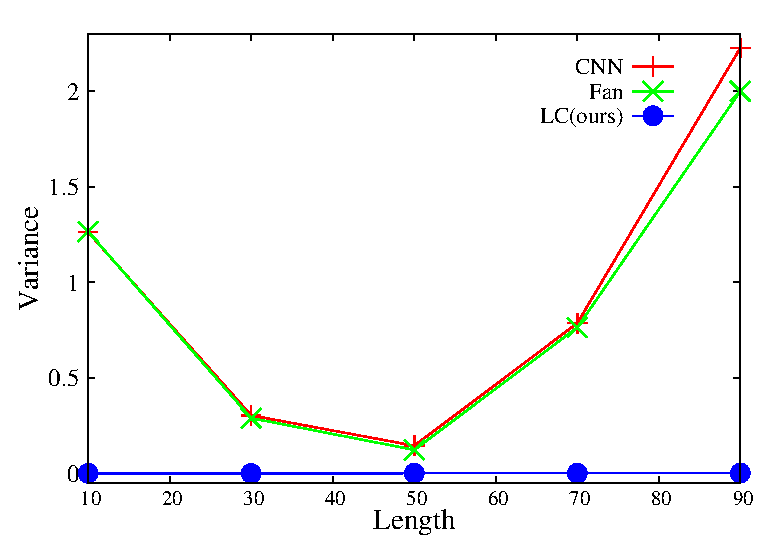
\includegraphics[width=2in]{VarF.eps}
  %\end{minipage}%
  }
  \subfigure[Variance in Trunc version]{
  \label{fig:varT}
  %\begin{minipage}[t]{0.5\linewidth}
    \centering
    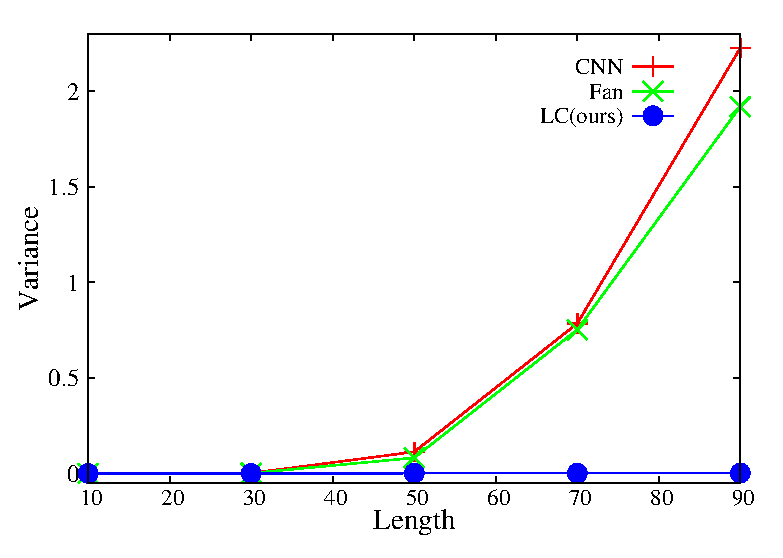
\includegraphics[width=2in]{VarT.eps}
  %\end{minipage}
  }
  \caption{Variance of different length}
  \label{fig:var}
\end{figure*}

\begin{table}[h]
	\centering
	\small
	\caption{Generated summaries of LC (Free) model}
	\label{tab:example}
	\begin{tabular}{|c|l}
	\hline
	\multicolumn{1}{c|}{\multirow{1}{*}{10}} &
	\tabincell{l}{
	    the \color{red}{younger jordan} \color{black}{was \textbf{rescued from his }}\\
		\textbf{disabled boat} .\\
	} 
	\\ \hline
	\multicolumn{1}{c|}{\multirow{1}{*}{30}} &
	\tabincell{l}{
	    \color{red}{louis jordan} \color{black}{was \textbf{rescued from his disabled }} . \\
		he \textbf{boat had n't been heard from in 66 days}\\
		\textbf{in late january} . he was rescued from his \\
		disabled boat . \\   
	} 
	\\ \hline
	\multicolumn{1}{c|}{\multirow{1}{*}{50}} &
	%\multicolumn{1}{c|}{Free} & 
	\tabincell{l}{ 
	   `` \textbf{i thought i lost you} , '' jordan says . the\\
	   \color{red}{younger jordan} \color{black}{was on \textbf{a sailboat a few miles}} \\
	   \textbf{off the south carolina coast} . `` i thought i lost \\
	   you , '' jordan tells \textbf{his son} . jordan says he was \\
	   grateful to the people .\\
	} 
	\\ \hline
\end{tabular}
\end{table}

To demonstrate the effectiveness of LC model and
 further illustrate the results,
we show an example of generated summaries by LC(Free) model 
with different lengths. 
%As is shown in \tabref{tab:example}, the summaries with different length have a high quality
%on both sematics and length controlling. 
As shown in \tabref{tab:example}, when the desired length (e.g., 10) is
very different from the length of the reference summary, the ROUGE score
may not be good even though the generated summary matches the reference
quite well semantically. The generated summaries from LC model are
{\em natural} and {\em complete}. 
The summaries with short desired length on Trunc and Exact version
would be more vulnerable to the incomplete problem. 
%It means that the sentences in summaries are readable and grammatical. 
We randomly sample 100 summaries generated by each model under 
Trunc and Exact with desired length of 10 and 30, and manually
inspect their readibility. This is a simplified human-evaluation 
of summarization, which just determines whether the sentences in summaries 
under length control are complete or not. If complete, the score is 1; 
if not, it is 0. It is easier to accomplish and more reliable
than other sophisticated human-evaluation.
\tabref{table:natural} shows that the LC model has a clear
advantage over the other two models in terms of summary fluency.

\begin{table}[th]
	\centering
	\small
	\caption{The proportion of summaries that are natural and complete with 
desired length 10 and 30}
	\label{table:natural}
	\begin{tabular}{p{1.8em}<{\centering}p{1.8em}<{\centering}p{1.8em}<{\centering}p{1.8em}<{\centering}p{1.8em}<{\centering}}%{|p{7cm}|rl|}
    \hline
    \multirow{2}{*}{}&
	\multicolumn{2}{c}{Trunc}&\multicolumn{2}{c}{Exact}\cr
	\cmidrule(lr){2-3} \cmidrule(lr){4-5} 
	& 10 & 30 & 10 & 30 \cr
	\hline
	CNN & 0.41 & 0.37 & 0.48 & 0.47\cr
	Fan & 0.50 & 0.42 & 0.53 & 0.57\cr
	LC & \bf 0.62 & \bf 0.59 & \bf 0.88 & \bf 0.86\cr
	\hline
    \end{tabular}
\end{table}


In this experiment, 
the desired length is fixed for all the documents which is independent from 
the corresponding lengths of reference summaries
%Besides, we can set different lengths to generation model for one source document. This makes the
such that the generated summaries may include more versatile 
words and phrases different from the reference summaries.
Thus, the similarity score is more reasonable for evaluation than 
ROUGE score.
As shown in \tabref{table:arbiSim} and \figref{fig:Sim}, 
the LC model achieves the highest similarity score
except for the length of $10$ and $30$ in the Free version.
The reason is that there is only 5\% of testing data with the length of reference summary shorter 
than 30. 
%If the generated summary is too short, the 
%similarity score will be small. This also causes the trends
%in \figref{fig:SimT} and \figref{fig:SimE}. 
Due to the effective length control of LC model,
the lengths of generated summaries from LC model are 
usually much shorter than those from the other models and 
the length of corresponding reference summaries
when we set the desired length as 10 or 30.
This leads to a relative lower similarity score shown in
\figref{fig:simT} and \figref{fig:simE}.
As shown in \figref{fig:var}, the LC model achieves the lowest
variance. 
In \figref{fig:varF}, as the length of most summaries is around
50 and the number of summaries with a length of 10 or 90 
is small, the CNN model and Fan model has lowest variance at 
50 and highest variance at 90.
In \figref{fig:varT}, the length of generated summaries in 
Trunc version is no more than desired length. So the variances
of CNN model and Fan model are incremental.
Besides, we can find that the LC model is stable under all 
conditions because of its effective length control model. 

%In , we can see that no one model can always be the best in the ROUGE score.
%So the ROUGE score can not reflect the quality of generated summary in this experiment. 
%Actually, the experiment 1 is the special case of experiment 2. 
%The problem (CNN and Fan 
%can get advantage in the Trunc version) in the 
%experiment 1 can also appears in experiment 2. 
%The repetition of the basic CNN seq2seq
%is still existed.
%Besides, we can set different lengths to generation model for one source document. This makes the
%generated summaries contain more words or phrase different from the reference summary.

%when the desired length is $10$, it is hard to match the reference summary
%for generated summaries. 
%However, the generated summaries can not match the reference summary
%well. 
%As the highest ROUGE scores are scattered in three models, 
%we should consider the similarity and variance. 
%It means LC model can effectively control the length of generated summary. 
%In the \figref{fig:Sim}, 
%the similarity score of LC model are better than others excepts length $10$ and $30$ in the Free version. 
%The reason is that the length of summaries generated by LC model is very close
%to $10$ or $30$. The generated summaries of other two models have longer length than $10$ 
%or $30$. The cosine similarity score tends to be small when the summary is too short.
%So this is a normal phenomenon.
%can generate summaries with setting length constraint.
%\tabref{ROUGE-maxlendiff}
% shows ROUGE score in different range with setting the max length
%of generated summaries as the max value in the range.
%As \label{ROUGE-maxlendiff} shows that our models can generate better
%summaries with any length range.
\subsection{Significance Test on Similarity Result}

We use significance test to prove that similarity metric is reliable 
even though the numerical difference of similarity scores in experiment
is little. Because the similarity scores of generated summaries do not follow
normal distribution, we take Kruskal-Wallis test \cite{loukina2014automatic,albert2017exploring} as our
significance test to measure that the difference of similarity results of three methods
is significant or not. As shown in \tabref{tab:pvalue}, all p-values are less than 0.05. 
The smaller p-value, the higher significant.
Thus, the difference of the similarity results is significant. 
%\YZ{table for significance test}

\begin{table}[th]
	\small
	\centering
	\caption{p-value of significance test}
	\label{tab:pvalue}
	\begin{tabular}{lcccc}
		\hline
		\multicolumn{1}{c}{}& Free & Trunc & Exact  \\ \hline
		\multicolumn{1}{c|}{Exp.1} & 3.4e-32 & 2.12e-45 & 0.01  \\ \cline{1-4}
		\multicolumn{1}{c|}{Exp.2} & 0.0 & 4.6e-39 & 1.0e-4  \\ \cline{1-4}
		\hline
	\end{tabular}
\end{table}

